\section{Specifika Krav}

\subsection{Funktionsmässiga krav}
\label{subsec:funcreq}

\subsubsection{Skärminspelning}
\begin{tabular}{ | p{65pt} | p{300pt} |}
  \hline
  Identifikator &
Skärminspelning
\\ \hline
  Beskrivning & 
Allt som användaren ser ska dokumenteras genom att ta så många bilder vi kan i sådan hög frekvens som möjligt.
  \\ \hline
  Motivering &
Applikationsutvecklaren måste få möjlighet att se hur användaren navigerar i applikationen för att se hur användarvänligt gränssnittet är.
  \\ \hline
  Behov &
Minimum
  \\ \hline
  Prioritet &  
Skärminspelningen har hög prioritet. Det är en av de viktigaste funktionerna för att få reda på hur användaren använder appen. En snabb prototyp behövs men skärminspelningsarbetet är tidsödande och behöver arbetas med konstant för att få ett så bra resultat som möjligt.
  \\ \hline
  Källa &
Dokument med krav från The Beta Family.
  \\ \hline
  Verifiering &
Kravet får verifieras genom att testa produkten på ett antal olika applikationer för att se att det fungerar att spela in skärmen oavsett vilken app som använder den.
  \\ \hline
\end{tabular}

\subsubsection{Röstinspelning}
\begin{tabular}{ | p{65pt} | p{300pt} |}
  \hline
  Identifikator &
Röstinspelning
  \\ \hline
  Beskrivning & 
  Vad användaren säger under testningen av applikationen ska spelas in.
  \\ \hline
  Motivering &
  Att höra användarens tankegångar under testning utav användargränssnitt är högst önskvärt av apputvecklare.
  \\ \hline
  Behov &
  Minimum
  \\ \hline
  Prioritet &
  Röstinspelningen har hög prioritet. Det är en av huvudfunktionerna och en av de funktioner som har tidigast deadline.
  \\ \hline
  Källa &
  Dokument med krav från The Beta Family.
  \\ \hline
  Verifiering &
  Kravet får verifieras genom att testa produkten på ett antal olika applikationer för att se att det fungerar att spela in ljud oavsett vilken app som använder den.
  \\ \hline
\end{tabular}

\subsubsection{Kamerainspelning}
\begin{tabular}{ | p{65pt} | p{300pt} |}
  \hline
  Identifikator &
  Kamerainspelning
  \\ \hline
  Beskrivning & 
  Användarens ansikte ska spelas in under testningen av applikationen
  \\ \hline
  Motivering &
  En visuell bild av användaren under testningen kan ge ytterligare information kring hur denna finner användarvänligheten.
  \\ \hline
  Behov &
  Minimum
  \\ \hline
  Prioritet &
  Kamerainspelningen har hög prioritet. Det är en av huvudfunktionerna och en av de funktioner som hr tidigast deadline.
  \\ \hline
  Källa &
  Dokument med krav från The Beta Family
  \\ \hline
  Verifiering &
  Kravet får verifieras genom att testa produkten på ett antal olika applikationer för att se att det fungerar att spela in från kameran oavsett vilken app som använder den.
  \\ \hline
\end{tabular}

\subsubsection{Användaren har själv kontroll över vad som spelas in}
\begin{tabular}{ | p{65pt} | p{300pt} |}
  \hline
  Identifikator &
  Användarkontroll
  \\ \hline
  Beskrivning & 
  När en person betatestar en app med hjälp utav The Beta Familys ScreenRecorder ska de kunna välja själv vad för information de vill ge utvecklarna. Testaren ska själv kunna bestämma om frontkameran och mikrofonen ska spela in under testet. 
  \\ \hline
  Motivering &
  Testaren bör kunna stänga av vissa funktioner då man inte alltid befinner sig i situationer då man är bekväm att t.ex. tala högljutt om vad som händer i appen. Det kan handla om att man gör ett test på tunnelbanan på vägen hem och bara vill visa hur man navigerar runt i applikationen.
  \\ \hline
  Behov &
  Standard
  \\ \hline
  Prioritet &
  Att användaren själv kan stänga av vissa funktioner är önskvärt men inte av högsta prioritet.
  \\ \hline
  Källa &
  Dokument med krav från The Beta Family
  \\ \hline
  Verifiering &
  En oberoende part får testa att genomföra ett test med olika funktioner avstängda. Lyckas personen utan problem stänga av önskade funktioner kan kravet anses uppfyllt och dessutom är det ett tecken på bra interaktionsdesign.
  \\ \hline
\end{tabular}

\subsubsection{Dubbeltryck för att få ner GUI:n}
\begin{tabular}{ | p{65pt} | p{300pt} |}
  \hline
  Identifikator &
  Dubbeltryck
  \\ \hline
  Beskrivning & 
  För att användaren ska få ner det grafiska gränssnittet ska hen göra ett s.k. dubbeltryck\emph{double tap} som innebär att man knackar två gånger med två fingrar på skärmen. Detta tar fram menyn för inspelningen där man kan starta och stoppa inspelningen samt ändra inställningar. Funktionen ska finnas oavsett var i applikationen man befinner sig.
  \\ \hline
  Motivering &
  The Beta Family har denna funktion i sin iOS-version och vill gärna att Android-versionen är så lik den som möjligt.
  \\ \hline
  Behov &
  Standard
  \\ \hline
  Prioritet &
  Det grafiska gränssnittet kan visa sig värdefullt att ha vid utveckling och testning av applikationen. Detta krav kommer antagligen implementeras rätt tidigt i utvecklingen så även om detta krav inte har högsta prioritet kommer det förhoppningsvis genomföras tidigt.
  \\ \hline
  Källa &
  The Beta Familys ScreenRecorder-SDK för iOS.
  \\ \hline
  Verifiering &
När projektet är klart implementeras SDK:n i en valfri applikation och sedan testas detta krav genom att dubbelknacka i olika lägen.
  \\ \hline
  \end{tabular}

\subsection{Tekniska krav och begränsningar}
\label{subsec:techreq}

\begin{figure}[H]
\centering
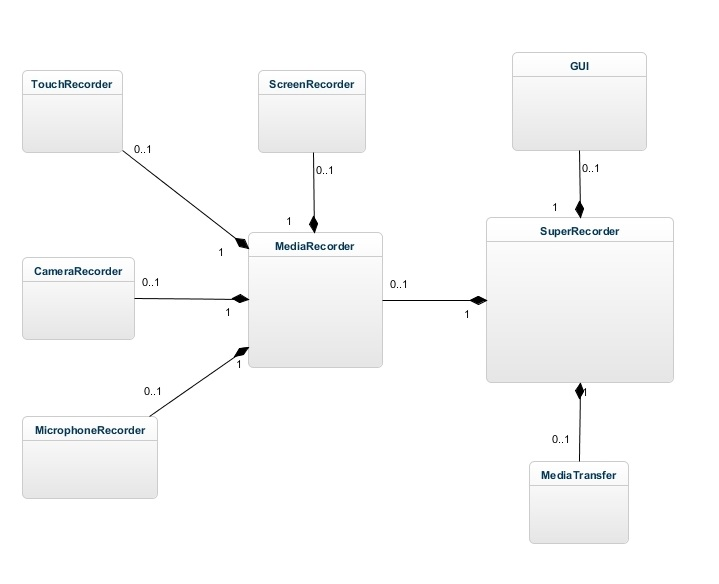
\includegraphics[width=\textwidth,height=\textheight,keepaspectratio]{SuperRecorderClassDiagram-diag.jpg}
\caption*{\textit{Klassdiagram för SuperRecorder}}
\label{figure:class}
\end{figure}

\subsubsection{Snabb implementation av SDK:n}
\begin{tabular}{ | p{65pt} | p{300pt} |}
  \hline
  Identifikator &
  Snabb SDK-implementation.
  \\ \hline
  Beskrivning & 
  Enligt The Beta Family kan deras ScreenRecorder för iOS implementeras på under två minuter av utvecklaren. Det är önskvärt att Androidversionen är lika simpel att implementera.
  \\ \hline
  Motivering &
  En del av The Beta Familys affärsidé är att utvecklarna själva implementerar deras ScreenRecorder. Detta ställer krav på utvecklaren att de kan implementera bibliotek och skriva några rader kod. Därför vill The Beta Family att implementationen är så simpel som möjligt. Krävs en mängd invecklade operationer och beslut kan detta skrämma bort eventuella kunder som då kanske väljer att inte betatesta applikationen.
  \\ \hline
  Behov &
  Standard
  \\ \hline
  Prioritet &
  Att SDK:n är simpel att genomföra har ganska hög prioritet. Det viktigaste är självklart att den funktionsmässigt fungerar. Om den är krånglig att implementera kan den fortfarande användas av mer tekniska utvecklare. En SDK som är simpel att implementera kommer leda till att fler utvecklare får värdefull återkoppling och väljer att använda The Beta Familys tjänst igen.
  \\ \hline
  Källa &
  Uppstartsmöte med The Beta Family där VD:n Axel Nordenström gick igenom krav.
  \\ \hline
  Verifiering &
  När projektet är färdigställts kan en oberoende part låtas implementera SDK:n på tid. Lyckas personen implementera SDK:n på under två minuter kan detta krav ses som uppfyllt.
  \\ \hline
\end{tabular}

\subsubsection{Testning ska kunna ske var som helst}
\begin{tabular}{ | p{65pt} | p{300pt} |}
  \hline
  Identifikator & 
  Platsoberoende tester
  \\ \hline
  Beskrivning & 
  Ett test ska kunna genomföras var som helst. Det ska inte krävas att mobilen är kopplad till en dator eller att det finns internetuppkoppling.
  \\ \hline
  Motivering &
  Genom att möjliggöra tester oberoende av plats och internetuppkoppling fås fler tester. En testare kan t.ex. genomföra ett test på tåget hem från jobbet. Utökar man mängden tillfällen ett test kan ske på ökar man också sannolikheten att testaren gör ett väl genomfört test då det sker på testarens villkor. Dessutom är detta ett viktigt krav för applikationer som beror på platsen. En applikation för Stockholms kommunaltrafik skulle inte kunna testas om det fanns krav på att mobilen var kopplad till datorn via sladd.
  \\ \hline
  Behov &
Minimum
  \\ \hline
  Prioritet &
Prioriteten är hög, detta är något som samtliga gruppmedlemmar måste ha i åtanke från första början av utvecklingen. Android tillåter en del extra funktioner om mobilen befinner sig i felsökningsläge och är kopplad till datorn via sladd. På grund av kravet på platsoberoende testning är det viktigt att utvecklarna redan från början tänker på att inte använda sig av dessa funktioner. Det kan vara svårt, om inte omöjligt, att anpassa sig efter kravet i efterhand.
  \\ \hline
  Källa &
 Uppstartsmöte med The Beta Family där VD:n Axel Nordenström gick igenom krav.
  \\ \hline
  Verifiering &
  Om ett test kan genomföras på en mobil med avstängd datatrafik, utan att vara kopplad till en dator, kan kravet anses vara uppfyllt.
  \\ \hline
\end{tabular}

\subsubsection{Inspelningen får inte försämra applikationens prestanda}
\begin{tabular}{ | p{65pt} | p{300pt} |}
  \hline
  Identifikator &
  Bibehållen prestanda
  \\ \hline
  Beskrivning & 
  Under inspelning ska applikationens prestanda ej påverkas.
  \\ \hline
  Motivering &
  Om inspelningen påverkar applikationens prestanda kan även testarens åsikter om applikationen påverkas. Detta kan leda till negativa åsikter om applikationen. Dessutom kan det innebära att utvecklarna lägger ner onödig tid på att leta prestandaproblem i sin applikation.
  \\ \hline
  Behov &
Standard
  \\ \hline
  Prioritet &
  Detta är något som måste has i åtanke från första början och lär påverka många designval under utvecklingsprocessen. Därför har detta krav hög prioritet.
  \\ \hline
  Källa &
  Kravspecifikation från The Beta Family
  \\ \hline
  Verifiering &
  En mängd prestandatunga applikationer kan testas vid projektets slut av oberoende testare. Märker dessa personer inte av en prestandaförsämring kan kravet anses uppfyllt.
  \\ \hline
\end{tabular}

\subsubsection{Fingerrörelser ska visas i realtid}
\begin{tabular}{ | p{65pt} | p{300pt} |}
  \hline
  Identifikator &
  Realtidsfingerrörelser
  \\ \hline
  Beskrivning & 
  The Beta Family är medvetna om att det finns en risk att testvideon kommer ha låg FPS. Fingerrörelser ska dock visas i realtid och inte begränsas till den FPS videon spelas upp i.
  \\ \hline
  Motivering &
  Om fingerrörelserna har samma låga FPS som videon blir det svårt att skilja enkla tryck från svepningar. Skulle man trycka flera gånger per sekund går dessutom flera rörelser förlorade.
  \\ \hline
  Behov &
  Standard
  \\ \hline
  Prioritet &
  Prioriteten är relativt hög då detta är en viktig del i att förstå hur användaren rör sig runt i applikationen.
  \\ \hline
  Källa &
  Uppstartsmöte med The Beta Family där VD:n Axel Nordenström gick igenom krav.
  \\ \hline
  Verifiering &
  Kravet verifieras när en testvideo kan presenteras där fingerrörelser visas oberoende av videons bildfrekvens.
  \\ \hline
\end{tabular}

\subsubsection{Androidenheten ska ej vara rootad}
\begin{tabular}{ | p{65pt} | p{300pt} |}
  \hline
  Identifikator &
  Ska ej vara rootad
  \\ \hline
  Beskrivning & 
  En Androidenhet som använder sig av SDK:t ska inte behöva vara rootad för att tester ska vara möjliga att genomföra.
  \\ \hline
  Motivering &
  Om enheten måste vara rootad för att ha möjligheten att använda SDK:t begränsas antalet kompatibla enheter drastiskt då de flesta androidenheter inte är rootade. Detta innebär även att antalet personer som kan testa applikationer minskar avsevärt. Kravet finns för att förenkla användningen av SDK:t både för utvecklare och testare.
  \\ \hline
  Behov &
  Minimum
  \\ \hline
  Prioritet &
  Prioriteten är hög då detta är ett av de primära kraven för SDK:n.
  \\ \hline
  Källa &
  Dokument med krav från The Beta Family.
  \\ \hline
  Verifiering &
  Kravet verifieras när projektet är färdigställt och kan testas på en androidenhet som inte är rootad.
  \\ \hline
\end{tabular}

\subsubsection{Gränssnittet ska vara så likt iOS-versionen som möjligt}
\begin{tabular}{ | p{65pt} | p{300pt} |}
  \hline
  Identifikator &
  Utseende likt iOS-versionen
  \\ \hline
  Beskrivning & 
  Den meny som användaren ska använda för att kontrollera ScreenRecorder:n ska vara så lik iOS-versionen som möjligt.
  \\ \hline
  Motivering &
  Det är positivt för företaget om dess produkter påminner om varandra. Detta skapar en känsla av igenkänning hos erfarna användare som nyttjat produkter från företaget tidigare.
  \\ \hline
  Behov &
  Deluxe
  \\ \hline
  Prioritet &
  Prioriteten är hög. Eftersom gränssnittet är något av det första som ska vara klart bör detta has i åtanke från första början.
  \\ \hline
  Källa &
  Dokument med krav från The Beta Family.
  \\ \hline
  Verifiering &
  Kravet verifieras genom att en oberoende part får jämföra Androidversionen med iOS-versionen.
  \\ \hline
\end{tabular}

\subsubsection{Stöd för att skicka sensordata i framtiden}
\begin{tabular}{ | p{65pt} | p{300pt} |}
  \hline
  Identifikator &
  Sensordata
  \\ \hline
  Beskrivning & 
  The Beta Family vill ha möjligheten att utöka funktionaliteten så att det går att skicka med data som samlas av mobilens sensorer. Ett exempel på en sensor är rörelsesensorn som mäter acceleration och rotation.
  \\ \hline
  Motivering &
  Ett stöd för sensordata gör mängden applikationer som kan testas större. Det finns t.ex. vissa spel som styrs genom att telefonen roteras.
  \\ \hline
  Behov &
  Deluxe
  \\ \hline
  Prioritet &
  Prioriteten är låg. Detta är något som projektgruppen måste ha i åtanke när SDK:t utvecklas men något som inte behöver göras tidigt.
  \\ \hline
  Källa &
  Uppstartsmöte med The Beta Family där VD:n Axel Nordenström gick igenom krav.
  \\ \hline
  Verifiering &
  Kravet verifieras om det lätt går att utöka den mängd information som skickas från mobilen till servern.
  \\ \hline
\end{tabular}

